%*************************************
% ภาคผนวก ข.
%*************************************
\appendixChapterTitle{ข}{คู่มือการใช้งานระบบ แบบสอบถาม และประวัติผู้จัดทำ}
\vspace{0.2in}

\section{คู่มือการใช้งานระบบ OrgChat AI (User Manual)}
\hspace*{1.3em}
ในส่วนนี้เป็นการอธิบายขั้นตอนการใช้งานระบบปัญญาประดิษฐ์แชทบอทสำหรับองค์กร OrgChat AI ตามขอบเขตการทำงานที่พัฒนาแล้วเสร็จในภาคการศึกษาที่ 1/2569 สำหรับกลุ่มผู้ใช้งาน 2 กลุ่ม ได้แก่ ผู้ดูแลระบบองค์กร (System Administrator) และพนักงานทั่วไป (Staff)

\subsection{การเข้าสู่ระบบและการจัดการสิทธิ์การใช้งาน (Authentication \& Access Control)}
\hspace*{1.3em}
ผู้ใช้งานสามารถเข้าถึงระบบเว็บแอปพลิเคชันได้ผ่านทางเว็บบราวเซอร์ โดยมีขั้นตอนการใช้งานดังนี้:
\begin{enumerate}[leftmargin=3.5em]
\item \textbf{การเข้าสู่ระบบด้วยบัญชีผู้ดูแลระบบ}: ผู้ดูแลระบบกรอกอีเมล (Email) และรหัสผ่าน (Password) ที่ได้รับจากระบบลงในแบบฟอร์มเข้าสู่ระบบ จากนั้นกดปุ่ม "เข้าสู่ระบบ (Sign In)" ดังแสดงในภาพที่ ข-1
\item \textbf{การเข้าสู่ระบบด้วย Google Sign-In}: พนักงานทั่วไปสามารถกดปุ่ม "เข้าสู่ระบบด้วย Google หรือสแกน QR Code" ระบบจะนำทางไปยังหน้าจอยืนยันตัวตนของ LINE Platform และส่งกลับมายังหน้าหลักของระบบโดยอัตโนมัติ
\item \textbf{การออกจากระบบ}: ผู้ใช้งานสามารถกดที่รูปโปรไฟล์มุมขวาบนของแถบเมนู และเลือก "ออกจากระบบ (Sign Out)" เพื่อทำลายเซสชันการใช้งานอย่างปลอดภัย
\end{enumerate}

\begin{figure}[htbp]
\centering
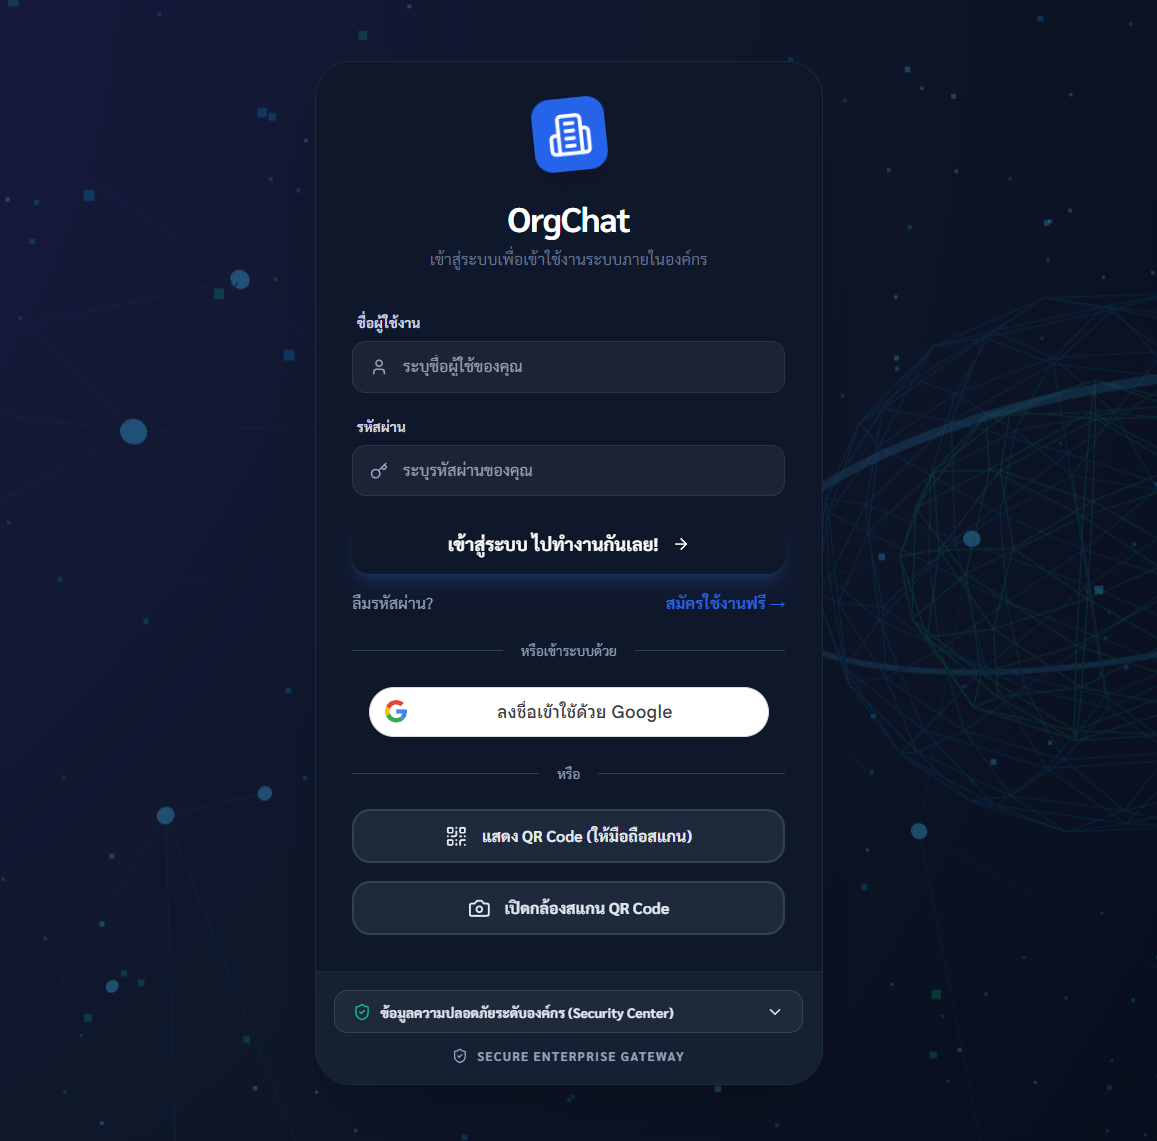
\includegraphics[width=0.88\textwidth]{Image/fig4_1_login.png}
\caption{หน้าจอเข้าสู่ระบบและสมัครสมาชิก OrgChat AI}
\label{figB:login}
\end{figure}

\subsection{การจัดการคลังความรู้องค์กร (Knowledge Base Management)}
\hspace*{1.3em}
ผู้ดูแลระบบสามารถจัดการเอกสารความรู้และคู่มือสินค้าของบริษัท ฮาร์ทวอมมิ่ง จำกัด เพื่อให้ AI สามารถนำไปใช้ตอบคำถามพนักงานได้ โดยมีขั้นตอนดังนี้:
\begin{enumerate}[leftmargin=3.5em]
\item \textbf{การเข้าสู่หน้าคลังความรู้}: เลือกเมนู "คลังความรู้ (Knowledge Base)" จากแถบเมนูด้านซ้ายของระบบเว็บแอปพลิเคชัน ดังแสดงในภาพที่ ข-2
\item \textbf{การอัปโหลดเอกสารใหม่}: 
  \begin{itemize}[leftmargin=2em]
    \item คลิกที่บริเวณพื้นที่อัปโหลดไฟล์ หรือลากไฟล์เอกสาร (รองรับไฟล์นามสกุล .pdf, .txt, .csv) มาวางในกรอบ
    \item ระบบจะตรวจสอบความถูกต้องของไฟล์ คำนวณค่าแฮช SHA-256 เพื่อตรวจจับไฟล์ซ้ำ และแสดงแถบความคืบหน้าของการอัปโหลด
    \item ระบบส่งไฟล์ไปจัดเก็บและสำรองไว้บนโฟลเดอร์ Google Drive ขององค์กรโดยอัตโนมัติ
  \end{itemize}
\item \textbf{กระบวนการประมวลผลเวกเตอร์ (Vector Indexing)}: ระบบจะทำการสกัดข้อความ ตัดแบ่งท่อนข้อมูล (Chunking) และแปลงเป็นเวกเตอร์เอ็มเบดดิงบันทึกลงสู่ ChromaDB สถานะเอกสารจะเปลี่ยนเป็น "พร้อมใช้งาน (READY)"
\item \textbf{การจัดการเอกสารเดิม}: ผู้ดูแลระบบสามารถตรวจสอบรายชื่อเอกสาร วันที่อัปโหลด ขนาดไฟล์ จำนวนท่อนข้อมูล (Chunks) และสามารถกดปุ่ม "ลบเอกสาร" เพื่อนำข้อมูลออกจากฐานข้อมูลเวกเตอร์ได้ทันที
\end{enumerate}

\begin{figure}[htbp]
\centering
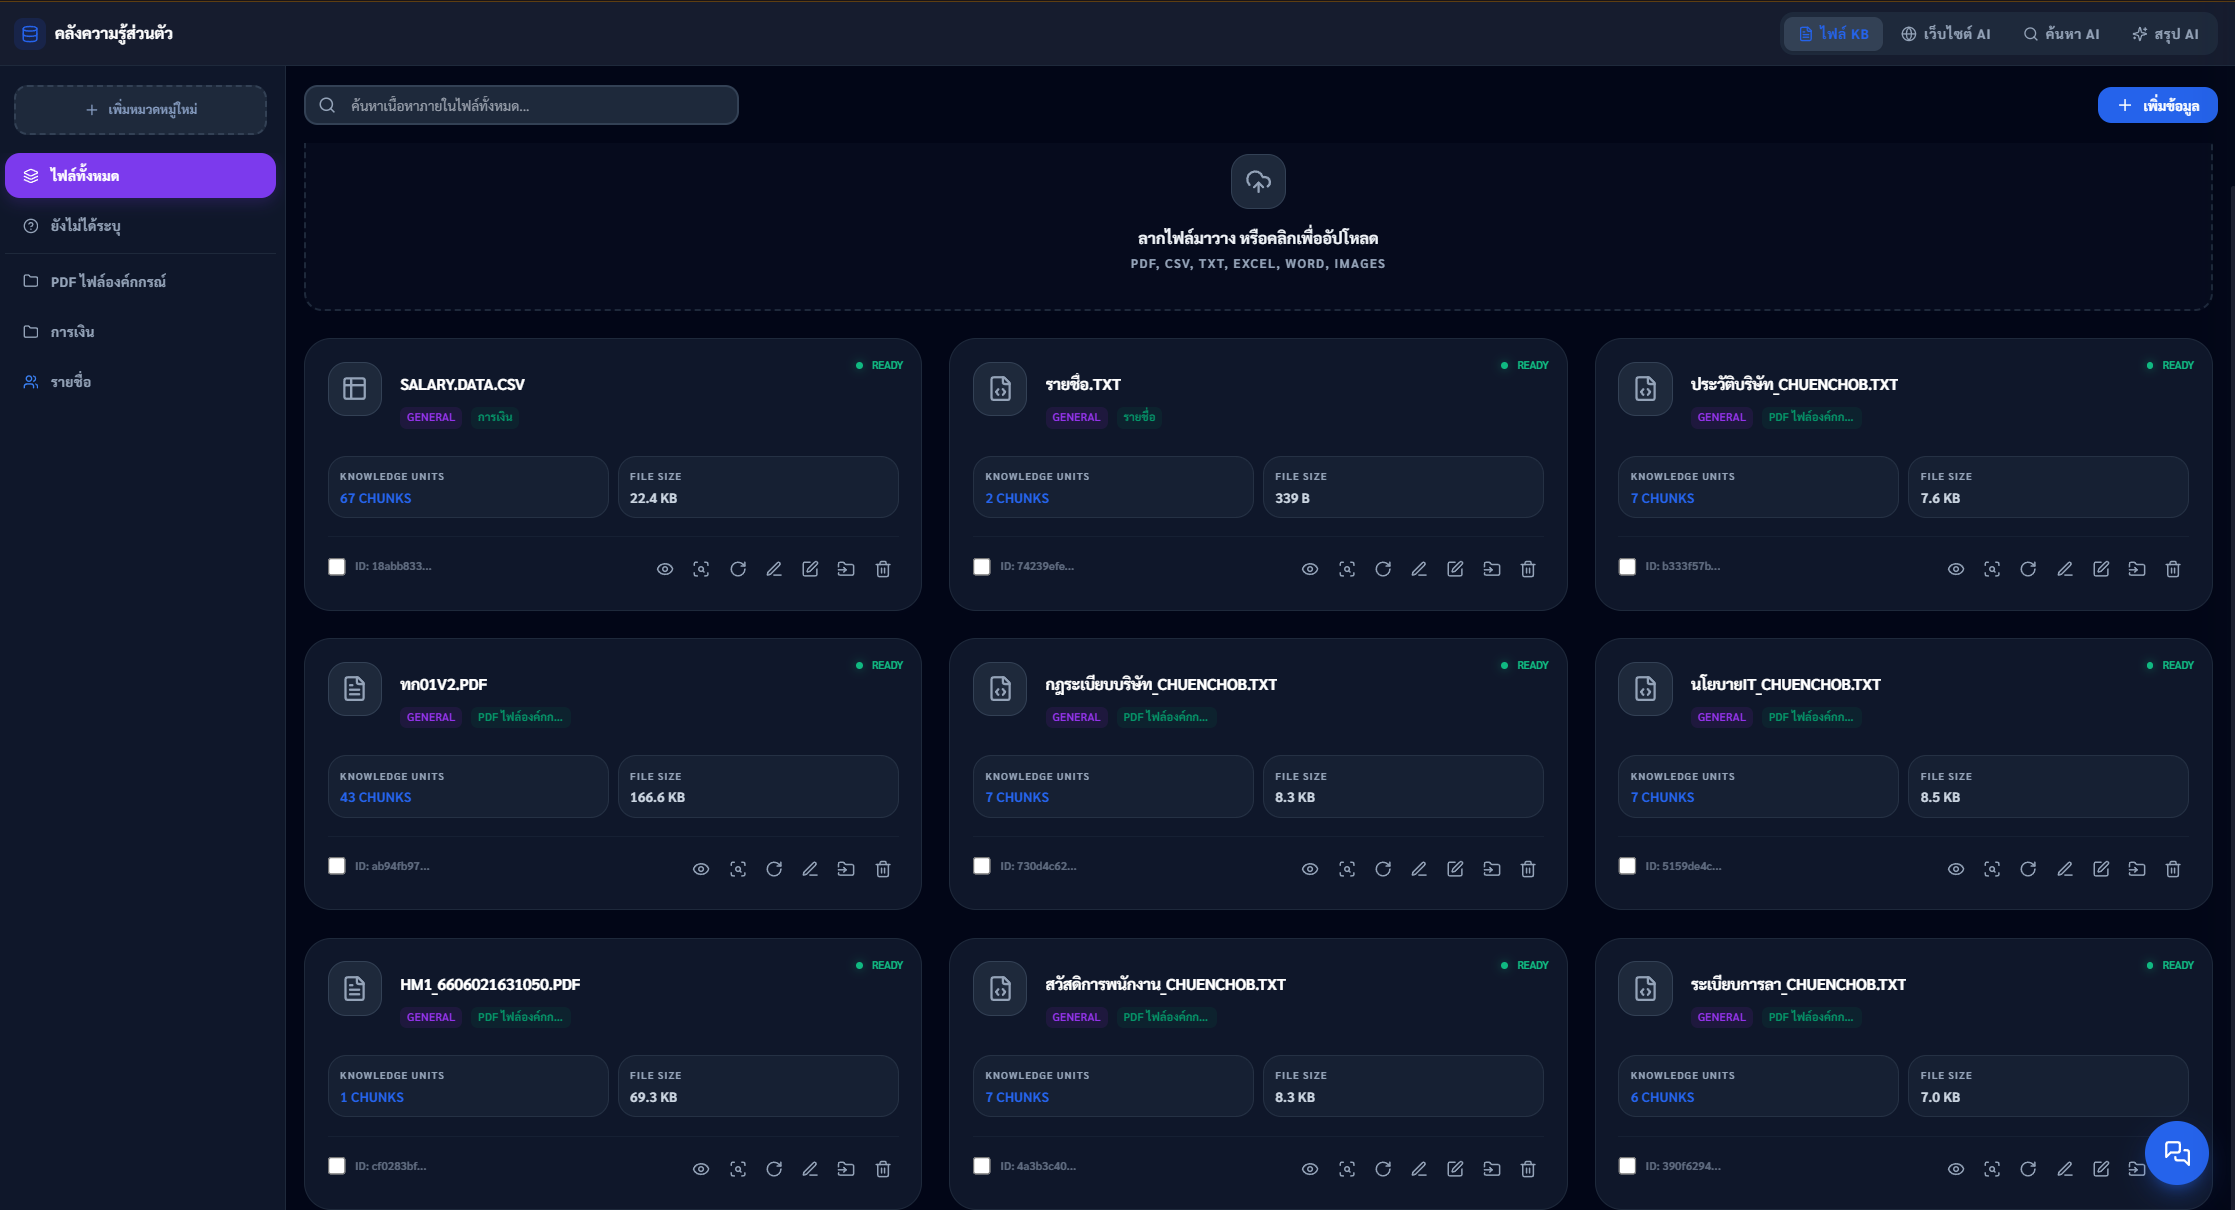
\includegraphics[width=0.88\textwidth]{Image/fig4_3_rag_kb.png}
\caption{หน้าจอการจัดการคลังความรู้องค์กรและการอัปโหลดเอกสาร}
\label{figB:rag_kb}
\end{figure}

\newpage
\subsection{การใช้งานแชทบอทผ่าน LINE Official Account (LINE Bot Interaction)}
\hspace*{1.3em}
พนักงานของบริษัท ฮาร์ทวอมมิ่ง จำกัด สามารถใช้งานผู้ช่วยอัจฉริยะในการสอบถามข้อมูลสินค้าและระเบียบปฏิบัติได้ทุกที่ทุกเวลาผ่านแอปพลิเคชัน LINE โดยมีขั้นตอนการใช้งานดังนี้:
\begin{enumerate}[leftmargin=3.5em]
\item \textbf{การเพิ่มเพื่อน}: สแกน QR Code หรือค้นหา LINE ID ของบัญชี LINE Official Account ของบริษัท และกดยืนยันการเพิ่มเพื่อน
\item \textbf{การพิมพ์คำถามภาษาธรรมชาติ}: พนักงานพิมพ์คำถามที่ต้องการทราบลงในช่องแชท เช่น \emph{"เงื่อนไขการรับประกันน้ำพุแมว duit เป็นอย่างไร"} หรือ \emph{"ถุงเท้าพิลาทิส thumb toe มีขนาดอะไรบ้าง"} ดังแสดงในภาพที่ ข-3
\item \textbf{การรับคำตอบจากแชทบอท}: ระบบจะค้นหาข้อมูลที่ตรงกันจากคลังความรู้และตอบกลับในรูปแบบการ์ด LINE Flex Message ที่จัดวางข้อความอย่างชัดเจน พร้อมแสดงแหล่งที่มาของเอกสารอ้างอิง
\item \textbf{การกดดูรายละเอียดเพิ่มเติม}: พนักงานสามารถกดปุ่มบนการ์ด Flex Message เพื่อเปิดดูเอกสารคู่มือฉบับเต็มบน Google Drive ได้โดยตรง
\end{enumerate}

\begin{figure}[htbp]
\centering
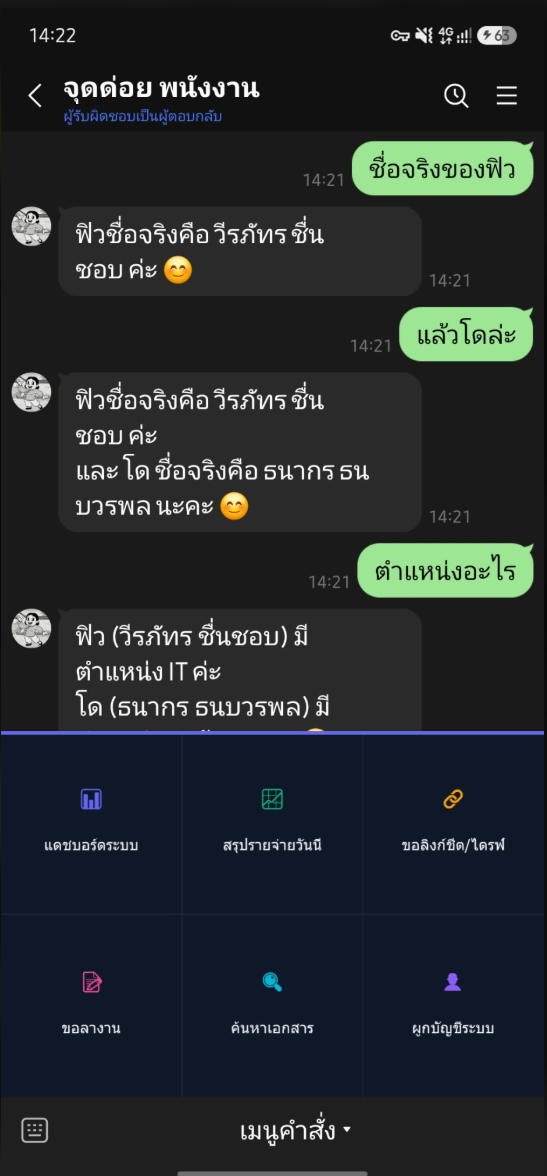
\includegraphics[height=0.42\textheight,keepaspectratio]{Image/fig4_2_line_rag.png}
\caption{การสนทนาสอบถามข้อมูลสินค้าผ่าน LINE Official Account}
\label{figB:line_rag}
\end{figure}

\subsection{การตรวจสอบประวัติการทำงานของระบบ (Audit Logs Inspection)}
\hspace*{1.3em}
ผู้ดูแลระบบสามารถตรวจสอบความโปร่งใสและความปลอดภัยของการใช้งานระบบ ผ่านหน้าจอบันทึกประวัติกิจกรรม (Audit Logs) ดังแสดงในภาพที่ ข-4:
\begin{enumerate}[leftmargin=3.5em]
\item เลือกเมนู "บันทึกกิจกรรม (Audit Logs)" จากแถบการนำทาง
\item ระบบจะแสดงตารางประวัติกิจกรรม ประกอบด้วย วันที่และเวลา, บัญชีผู้ใช้งาน, หมายเลข IP Address, ประเภทกิจกรรม (เช่น LOGIN, UPLOAD\_DOCUMENT, DELETE\_DOCUMENT) และสถานะผลลัพธ์
\item มีแถบค้นหาและตัวกรองตามช่วงเวลาและประเภทกิจกรรม เพื่อช่วยให้ผู้ดูแลระบบสามารถตรวจสอบความผิดปกติได้อย่างรวดเร็ว
\end{enumerate}

\begin{figure}[htbp]
\centering
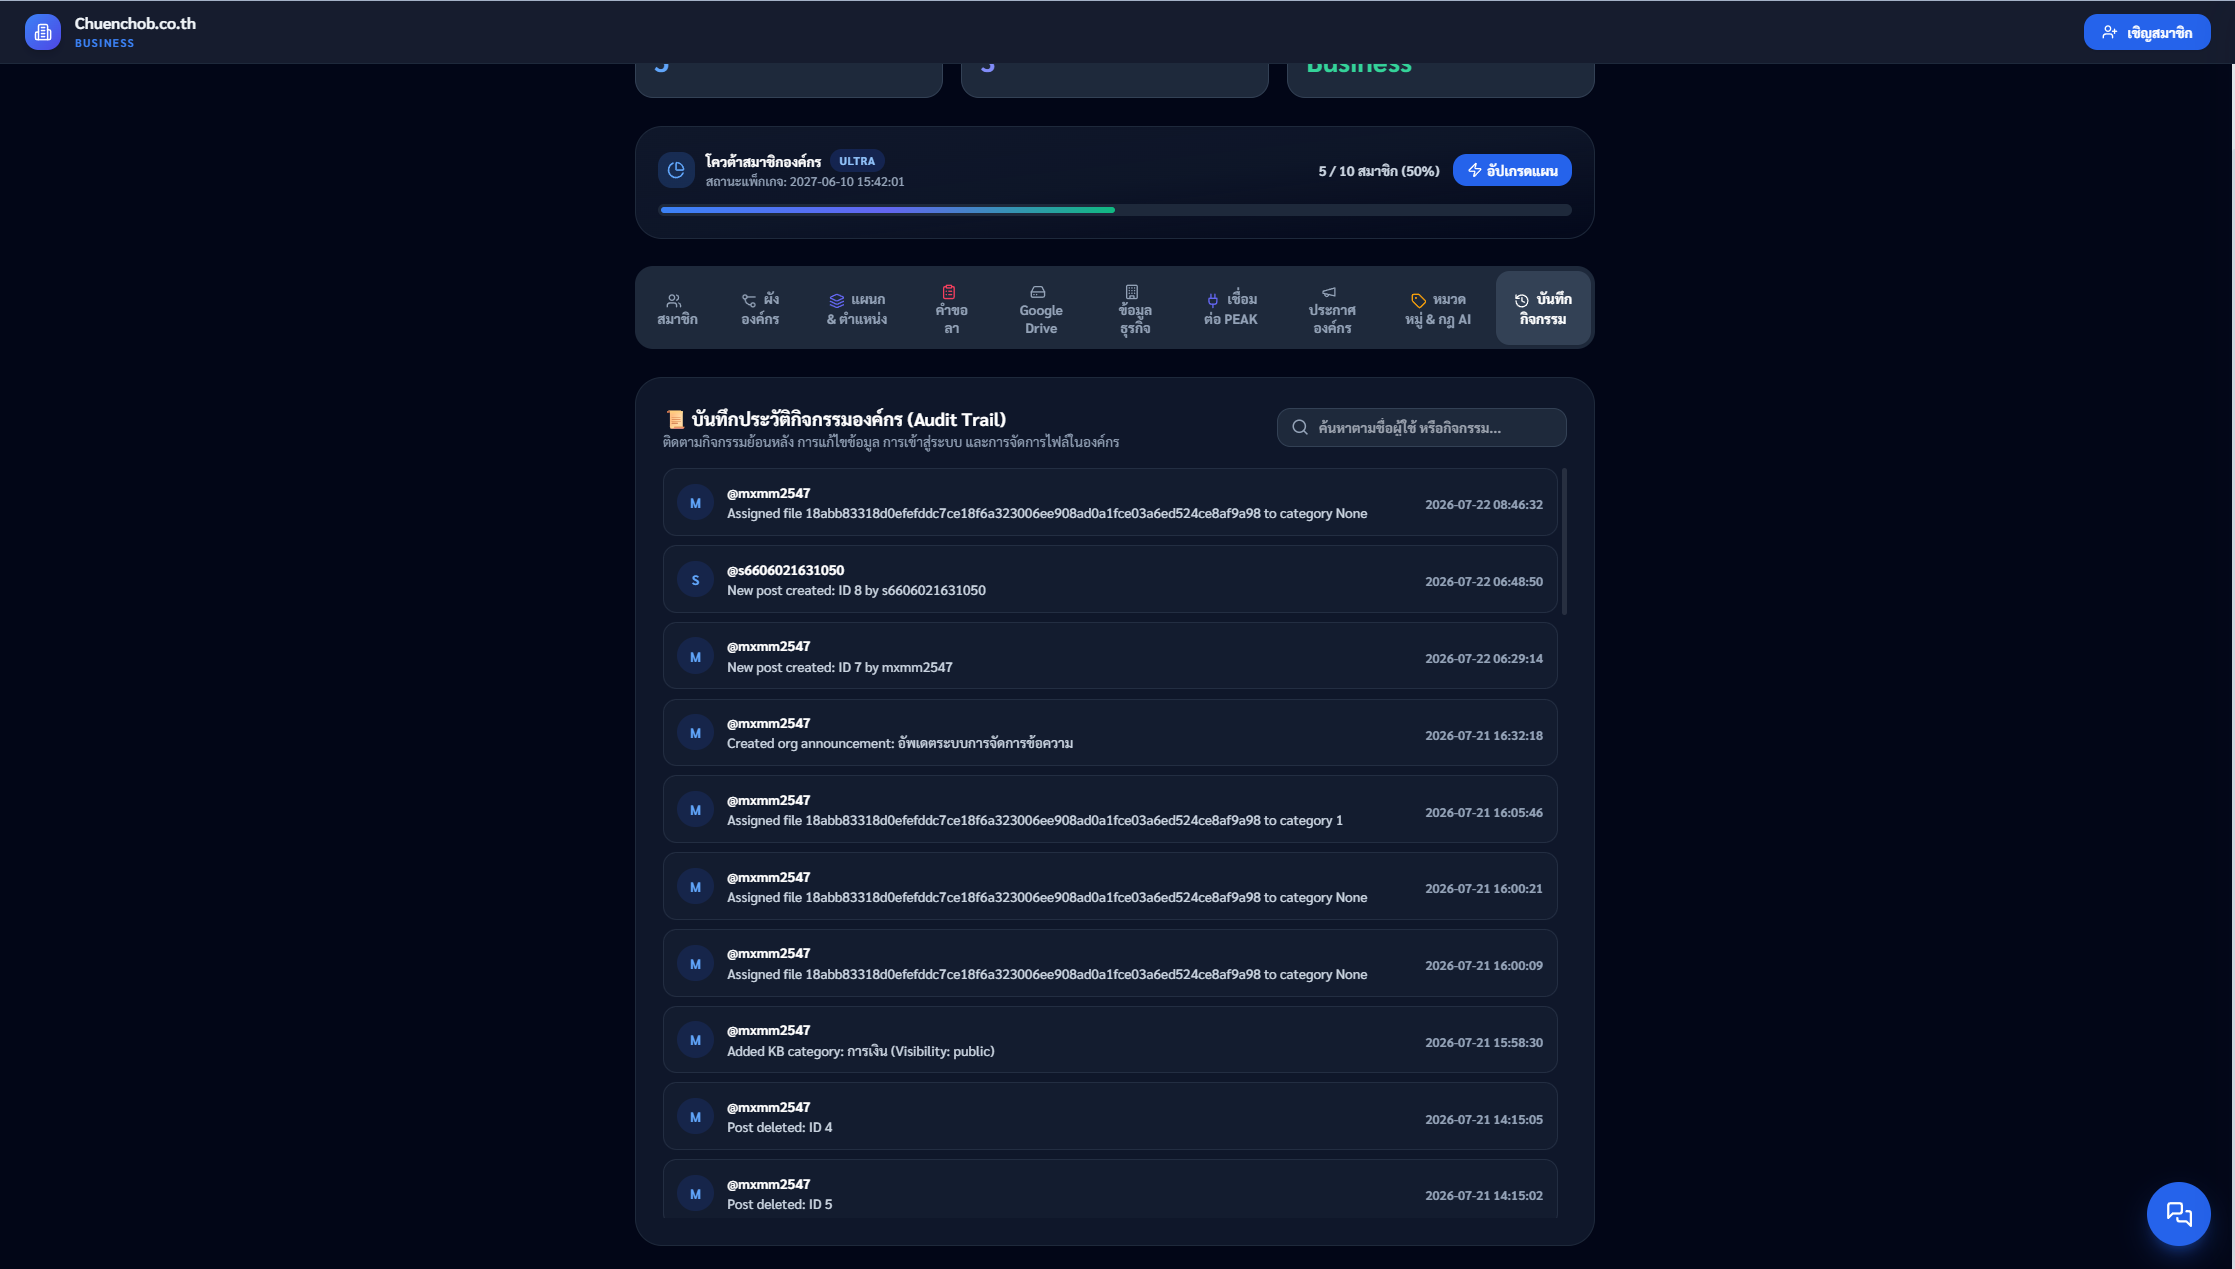
\includegraphics[width=0.88\textwidth]{Image/fig4_9_audit.png}
\caption{หน้าจอบันทึกประวัติการทำงานของระบบ (Audit Logs)}
\label{figB:audit}
\end{figure}

\newpage
\section{แบบร่างเครื่องมือประเมินความพึงพอใจสำหรับการดำเนินงานในภาคการศึกษาที่ 2/2569}
\hspace*{1.3em}
ในภาคการศึกษาที่ 2/2569 คณะผู้จัดทำมีแผนการนำระบบที่พัฒนาเสร็จสมบูรณ์ไปติดตั้งและทดสอบการใช้งานจริงร่วมกับบุคลากรของ บริษัท ฮาร์ทวอมมิ่ง จำกัด จำนวน 20 คน โดยจะใช้แบบสอบถามวัดความพึงพอใจตามมาตราส่วนประเมินค่า 5 ระดับของ Likert (Likert 5-Point Rating Scale) ซึ่งมีรายละเอียดของแบบร่างเครื่องมือดังแสดงในตารางที่ ข-1:

\vspace{0.5em}
\hspace*{1.3em}
\textbf{คำชี้แจง}: โปรดทำเครื่องหมาย $\checkmark$ ลงในช่องที่ตรงกับระดับความคิดเห็นของท่าน (5 = มากที่สุด, 4 = มาก, 3 = ปานกลาง, 2 = น้อย, 1 = น้อยที่สุด)

\begin{table}[htbp]
\centering
\caption{แบบร่างแบบสอบถามประเมินความพึงพอใจของผู้ใช้งานในภาคการศึกษาที่ 2/2569}
\label{tabB:survey}
\begin{tabularx}{\textwidth}{| c | L | c | c | c | c | c |}
\hline
\textbf{ข้อ} & \textbf{รายการประเมินความพึงพอใจ} & \textbf{5} & \textbf{4} & \textbf{3} & \textbf{2} & \textbf{1} \\ \hline
\multicolumn{7}{|l|}{\textbf{ด้านการออกแบบและการเข้าใช้งาน (Design and Usability)}} \\ \hline
1 & ความสะดวกและรวดเร็วในการเข้าใช้งานระบบผ่านแอปพลิเคชัน LINE & & & & & \\ \hline
2 & ความสวยงามและความชัดเจนของข้อความตอบกลับ LINE Flex Message & & & & & \\ \hline
3 & ความง่ายในการใช้งานหน้าจอเว็บแอปพลิเคชันสำหรับผู้ดูแลระบบ & & & & & \\ \hline
\multicolumn{7}{|l|}{\textbf{ด้านฟังก์ชันการทำงานและความถูกต้อง (Functionality and Accuracy)}} \\ \hline
4 & ความถูกต้องและตรงประเด็นในการตอบคำถามของระบบ RAG จากเอกสารคู่มือสินค้า & & & & & \\ \hline
5 & ความแม่นยำในการอ่านและสกัดข้อมูลจากภาพถ่ายสลิปโอนเงินด้วย OCR & & & & & \\ \hline
6 & ความสะดวกในขั้นตอนการยื่นคำขอลางานและการอนุมัติใบลาผ่าน LINE & & & & & \\ \hline
7 & ความครบถ้วนและประโยชน์ของข้อมูลสถิติบนแผงควบคุมผู้บริหาร (Dashboard) & & & & & \\ \hline
\multicolumn{7}{|l|}{\textbf{ด้านประโยชน์และความพึงพอใจในภาพรวม (Overall Benefits)}} \\ \hline
8 & ระบบช่วยลดระยะเวลาและขั้นตอนในการทำงานประจำวันของพนักงาน & & & & & \\ \hline
9 & ระบบช่วยลดข้อผิดพลาดในการรวบรวมข้อมูลและการสื่อสารภายในองค์กร & & & & & \\ \hline
10 & ความพึงพอใจในภาพรวมต่อการนำระบบ OrgChat AI มาช่วยปฏิบัติงาน & & & & & \\ \hline
\end{tabularx}
\end{table}

\newpage
\section{ประวัติผู้จัดทำโครงงาน (Author Biographies)}
\vspace{0.5em}

\subsection{นายธนากร ธนบวรพล (Mr. Thanakorn Thanabowonphon)}
\begin{mycustomitem}
\item \textbf{รหัสนักศึกษา}: 66-060-216-10117
\item \textbf{วัน เดือน ปีเกิด}: 15 กรกฎาคม พ.ศ. 2546
\item \textbf{สาขาวิชา}: สาขาวิชาเทคโนโลยีสารสนเทศ ภาควิชาเทคโนโลยีสารสนเทศ
\item \textbf{คณะ}: คณะเทคโนโลยีและการจัดการอุตสาหกรรม มหาวิทยาลัยเทคโนโลยีพระจอมเกล้าพระนครเหนือ (วิทยาเขตปราจีนบุรี)
\item \textbf{ประวัติการศึกษา}:
  \begin{itemize}[leftmargin=2em,noitemsep,topsep=2pt]
    \item พ.ศ. 2565: สำเร็จการศึกษาระดับมัธยมศึกษาตอนปลาย แผนการเรียนวิทยาศาสตร์-คณิตศาสตร์
    \item พ.ศ. 2566--ปัจจุบัน: กำลังศึกษาระดับปริญญาตรี หลักสูตรวิทยาศาสตรบัณฑิต สาขาวิชาเทคโนโลยีสารสนเทศ คณะเทคโนโลยีและการจัดการอุตสาหกรรม มจพ. ปราจีนบุรี
  \end{itemize}
\item \textbf{หน้าที่ความรับผิดชอบในโครงงาน}:
  \begin{itemize}[leftmargin=2em,noitemsep,topsep=2pt]
    \item วิเคราะห์และออกแบบระบบงานตามความต้องการของ บริษัท ฮาร์ทวอมมิ่ง จำกัด
    \item ออกแบบแผนภาพระบบ แผนภาพกระแสข้อมูล (DFD Level 0-2) และสถาปัตยกรรมระบบ
    \item ออกแบบแบบจำลองความสัมพันธ์ของข้อมูล (ER Diagram) และโครงสร้างตารางฐานข้อมูล SQLite
    \item พัฒนาระบบยืนยันตัวตน (Authentication) และระบบควบคุมสิทธิ์ตามบทบาท (RBAC)
    \item ออกแบบและเชื่อมต่อบริการ Google Drive API สำหรับจัดเก็บเอกสารองค์กร
    \item จัดทำเอกสารข้อกำหนดระบบ พจนานุกรมข้อมูล และจัดทำรายงานปริญญานิพนธ์
  \end{itemize}
\end{mycustomitem}

\newpage
\subsection{นายวีรภัทร ชื่นชอบ (Mr. Weeraphat Chuenchob)}
\begin{mycustomitem}
\item \textbf{รหัสนักศึกษา}: 66-060-216-31050
\item \textbf{วัน เดือน ปีเกิด}: 24 กันยายน พ.ศ. 2546
\item \textbf{สาขาวิชา}: สาขาวิชาเทคโนโลยีสารสนเทศ ภาควิชาเทคโนโลยีสารสนเทศ
\item \textbf{คณะ}: คณะเทคโนโลยีและการจัดการอุตสาหกรรม มหาวิทยาลัยเทคโนโลยีพระจอมเกล้าพระนครเหนือ (วิทยาเขตปราจีนบุรี)
\item \textbf{ประวัติการศึกษา}:
  \begin{itemize}[leftmargin=2em,noitemsep,topsep=2pt]
    \item พ.ศ. 2565: สำเร็จการศึกษาระดับมัธยมศึกษาตอนปลาย แผนการเรียนวิทยาศาสตร์-คณิตศาสตร์
    \item พ.ศ. 2566--ปัจจุบัน: กำลังศึกษาระดับปริญญาตรี หลักสูตรวิทยาศาสตรบัณฑิต สาขาวิชาเทคโนโลยีสารสนเทศ คณะเทคโนโลยีและการจัดการอุตสาหกรรม มจพ. ปราจีนบุรี
  \end{itemize}
\item \textbf{หน้าที่ความรับผิดชอบในโครงงาน}:
  \begin{itemize}[leftmargin=2em,noitemsep,topsep=2pt]
    \item ศึกษา วิจัย และพัฒนาระบบคลังความรู้อัจฉริยะ (RAG Pipeline) ด้วย ChromaDB และ FastEmbed
    \item พัฒนาระบบตัดแบ่งท่อนข้อมูล (Text Chunking) และสกัดข้อมูลจากเอกสารคู่มือสินค้า
    \item เชื่อมต่อและปรับแต่งโมเดล Google Gemini 1.5 Flash API สำหรับสังเคราะห์คำตอบภาษาธรรมชาติ
    \item พัฒนาระบบแชทบอท LINE Official Account ผ่าน LINE Messaging API Webhook
    \item ออกแบบและพัฒนาการแสดงผลข้อมูลด้วยการ์ด LINE Flex Message แบบ Interactive
    \item ดำเนินการทดสอบการทำงานของระบบ (Functional Black-Box Testing) และบันทึกผลการดำเนินงาน
  \end{itemize}
\end{mycustomitem}
